\chapter{Architettura di Sistema}\label{cap:Architettura}

%\begin{minipage}{12cm}\textit{Se lo si desidera, utilizzare questo spazio per inserire un breve riassunto di ci\`o che verr\`a detto in questo capitolo. Inserire solo i punti salienti.}
%\end{minipage}

%\vspace*{1cm}

\section{Architettura ad alto livello}
Il progetto finale ha come obiettivo la realizzazione di un architettura di controllo per le bobine poloidali presenti nei reattori tokamak.

\begin{figure}[h]
	\centering
	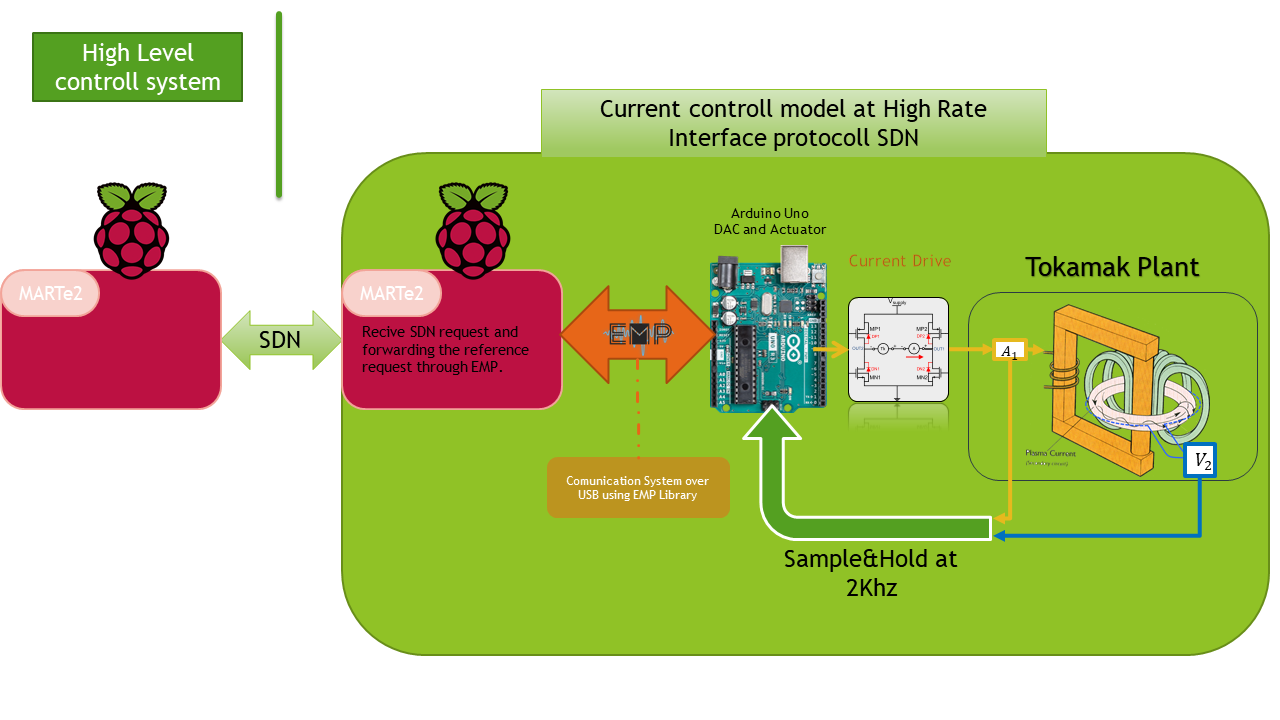
\includegraphics[width=1\textwidth]{Architettura/SystemArchitetture.png}
	\caption[Schema finale dell'archiettettura di controllo]{Architettura di controllo}
\end{figure}

\noindent
Lo schema proposto realizza l'obiettivo è controllare una singola bobina, il progetto finale prevederà la ripetizione in serie del medesimo schema per il numero di bobine necessarie.\\

Dallo schema risulta evidente che tutti i componenti visti nel capitolo "\nameref{cap:1}" si relazionano con lo stesso \microControllore: l'\ArduinoUno.\\
Per riportare i dati fuori e ricevere il riferimento da inseguire nella $V_2$, è stata realizzato il \nameref{EMP}, essa è stata scritta in C++ affinché possa essere Cross-Platform.\\
Il suo compito specifico, in questo progetto, è di mettere in comunicazione l'\ArduinoUno con un nodo \MARTe installato su di una \Rasp.\\
Quest'ultimo nodo ha il compito di mettere in rete il feedback dell'esperimento, e comunicare all'\ArduinoUno eventuali cambio di riferimento. Questo ultimo tratto è realizzato mediante il protocollo \textbf{SDN}, che viaggia sopra Ethernet e dà garanzie Real-time.\\
Nella sua forma finale, il progetto prevede la riproduzione in serie di questo schema di controllo per arrivare a controllare tutte le bobine poloidali presenti in un tokamak.

\newpage

\section*{EMP - Libreria di Comunicazione Seriale\\Embedded Message Pack }\label{EMP}
\addcontentsline{toc}{section}{\protect\numberline{\thesection} EMP - Libreria di Comunicazione Seriale}

\begin{figure}[h]
	\centering
	
\includegraphics[width=1\textwidth]{EMP/EMP-Logo-Background.png}
\end{figure}
\paragraph{EMP (Embedded Message Pack)} nasce con l’obiettivo di standardizzare un protocollo e creare una libreria C++ basata su classi Template, che permetta di automatizzare e standardizzare tutto il lavoro di programmazione necessario all’invio/ricezione di dei pacchetti dal formato Pre-Concordati tra 2 Device connessi Peer2Peer (Nessuna pretesa di network-ing).\\
Il raggiungimento dei suoi obiettivi, si sposa con la possibilità di supportare altre features interessanti:

\paragraph{Multiple-Package} Il protocollo di comunicazione che si è deciso di usare per EMP ha permesso di estendere il suo funzionamento e permettere il trasporto, attraverso lo stesso mezzo, di \textit{\textbf{pacchetti di tipologia e dimensione diversa}} all’interno della stessa libreria, evitando al contempo di inviare per ogni pacchetto più byte di quelli strettamente necessario. $\Rightarrow$ \textbf{Alta Efficienza}

\paragraph{Zero Tempo di negoziazione} Sempre grazie al protocollo di comunicazione, EMP è adatto ad un uso ‘Streaming’, questo perché non è necessario alcuna fase di sincronizzazione iniziale o durante la trasmissione in caso di perdita di dati, in aggiunta a ciò, EMP è in grado di scartare pacchetti errati in maniera trasparente all’utilizzatore. Tutto questo grazie al protocollo che \textbf{Auto-delimita i singoli pacchetti}. $\Rightarrow$ \textbf{Trasparenza Totale}

\paragraph{Responsabilità} Le uniche responsabilità a carico degli utilizzatori sono il riempimento dei pacchetti e la definizione degli stessi tra i 2 estremi della comunicazione.

\subsection*{Consistent Overhead Byte Stuffing (COBS)}
\addcontentsline{toc}{section}{\protect\numberline{\thesection} Protocollo - COBS}
Il protocollo di comunicazione che permette l’invio di \textbf{pacchetti diversi} e \textbf{senza fasi di negoziazione} alla base della libreria è \textbf{COBS}(\cite{COBS}).\\
Si tratta di un algoritmo per la codifica di byte, progettato per essere al tempo stesso efficiente e non ambiguo, che permette la definizione di \textit{data-pack frame} \textbf{Auto-delimiti} .

\begin{figure}[h]
	\centering
	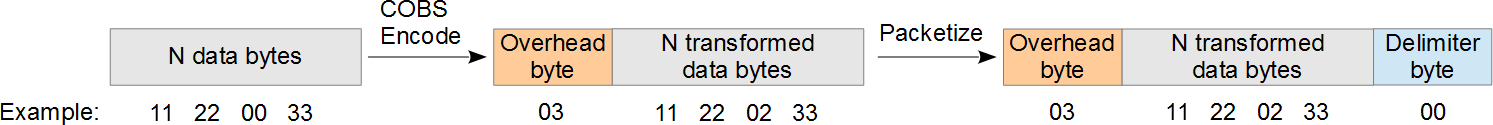
\includegraphics[width=1\textwidth]{EMP/Cobs_encoding_with_example.png}
	\caption[Esempio di COBS]{Esempio di COBS}
\end{figure}

\subsection{Metodo di codifica}
L'algoritmo di COBS trasforma una stringa arbitraria di byte, ciascuno dei quali ha un Range di valori da \textbf{[0:255]} in una nuova stringa di byte dove però ogni byte va da \textbf{[{\color{red}1}:255]}. La dimensione della nuova stringa è sempre pari alla dimensione della precedente + 1.\\
L'obiettivo di questo metodo di codifica è di eliminare tutti i possibili byte \zeroByte dal pacchetto in maniera reversibile.\\
Questo processo rende il carattere \textbf{\zeroByte (byte zero)} ottimo candidato per essere usato come terminatore di stringa durante l'invio, rendendo un pacchetto COBS-Encoded mai ambiguo e sempre \textbf{Auto-delimitato}.\\
L'algoritmo di codifica consiste nel:
\begin{enumerate} [itemsep=-3mm]
	\item Inserire un byte \zeroByte all'inizio del pacchetto
	\item Individuare tutti gli altri byte \zeroByte
	\item Inserire un byte \zeroByte alla fine del pacchetto
	\item Sostituire tutti gli \zeroByte con la distanza dal successivo \zeroByte nella stringa, ignorando l'ultimo
\end{enumerate}

\begin{figure}[h]
	\centering
	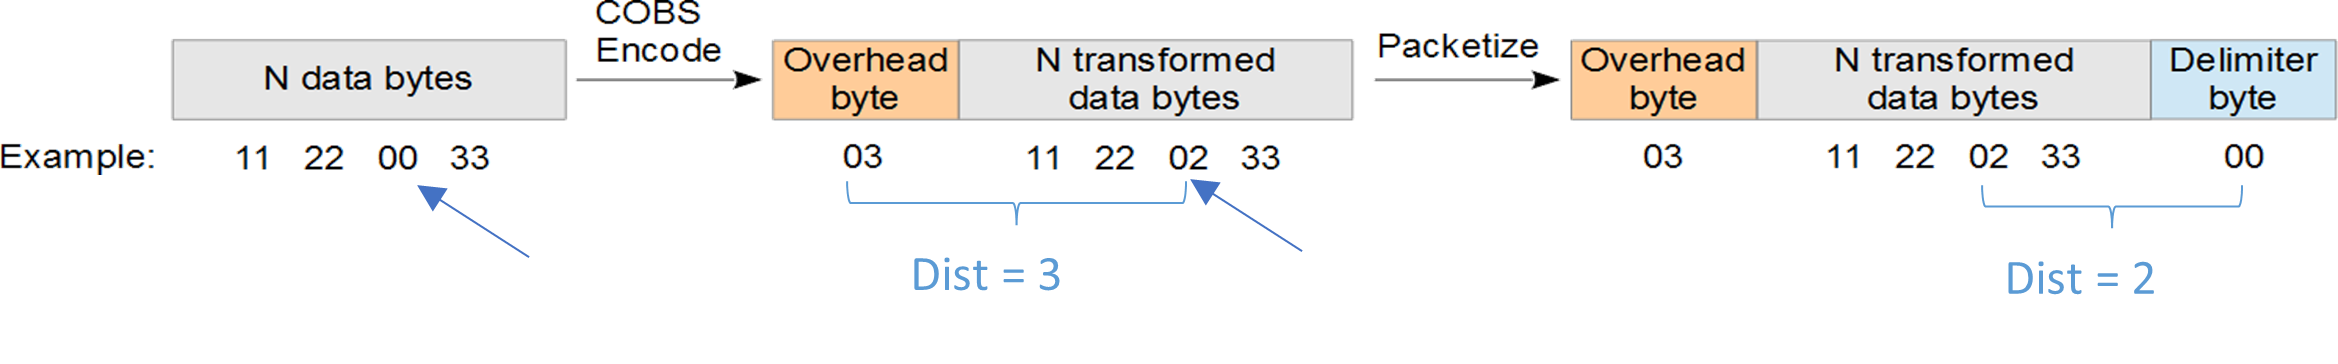
\includegraphics[width=1\textwidth]{EMP/Cobs_encoding_with_example-dist.png}
	\caption[Esempio di COBS con distanza]{Esempio di COBS con distanza}
\end{figure}

La versione usata per questo progetto, che comunque non ha l'obiettivo di trasmettere quantità infinite di byte, ha il limite di non poter codificare blocchi di byte che hanno una distanza tra 2 \zeroByte superiore a 255, questo limite è potenzialmente rimovibile usando un algoritmo più sofisticato.

\subsection{Struttura del codice}

\subsection{Benchmark}

\newpage
\section{Online Sampling}
\subsection{Interconnessione Arduino $\Leftrightarrow$ Companion}
\subsection{Storage su file delle informazioni}

\newpage
\section{Post Elaborazione con Matlab}
\subsection{Conversioni Dati}
\subsection{Creazione dei grafici e Filtraggio}
